% intro 
The simulations of blood flows in nozzle, pump, and IVC with FEM and PFEM-2 are conducted and compared with experimental results in \cite{fda_res}, \cite{fda_nozzle}, \cite{fda_pump} and \cite{gallagher_exp}. The fluid is assumed to be Newtonian blood analog fluid. For the nozzle and pump flows, the fluid density and viscosity are $\rho= 1035$ kg/m\textsuperscript{3} and $\mu =3.5\times10^{-3}$ N-s/m\textsuperscript{2}, where as for the flow in IVC, the density and viscosity are $\rho=1817$ kg/m\textsuperscript{3}, $\mu=5.83\times10^{-3}$ N-s/m\textsuperscript{2} for resting condition and $\mu=5.49\times10^{-3}$ N-s/m\textsuperscript{2} for exercising condition. 

\subsection{Nozzle}

%  nozzle intro
The simplified nozzle proposed by FDA consists of four parts containing characteristics of some blood-conveying medical devices. There are inlet and outlet tubes with diameter $0.012$ m, as well as a cone-shaped converging tube connecting the inlet tube with the nozzle throat with diameter $0.004$ m as shown in figure~\ref{fig:nozzlegeo1}. The flow experiences a gradual contraction of area from the inlet tube to the throat, then a sudden expansion of the area right after the throat to the outlet tube (figure~\ref{fig:nozzlegeo2}). It is set that the z cordinate along the axial direction has origin at the exit of the nozzle throat. The flow with Reynolds number $3500$ with flowrate $3.64\times10^{-5}$ m\textsuperscript{3}/s corresponding to turbulent flow regime is analyzed, where the Reynolds number is defined with the flow rate and the diameter at the throat. 

%% PEGGY: should these geometry figures be included?
\begin{figure}[htbp]
    \centering
    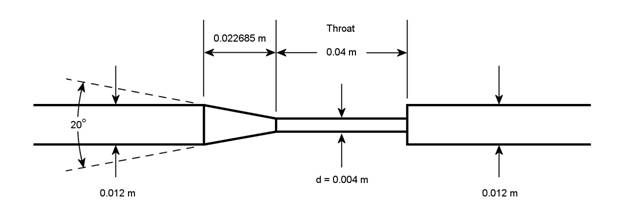
\includegraphics[width=3.2in]{imgs/nozzle_pump/nozzle_geo.jpg}
    \caption{The dimension of the idealized nozzle model proposed by FDA.}
    \label{fig:nozzlegeo1}
\end{figure}
\begin{figure}[htbp]
    \centering
    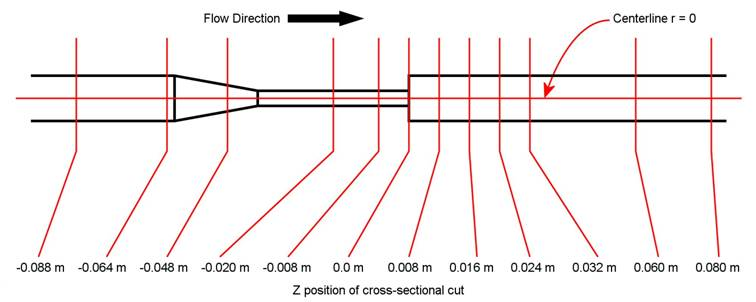
\includegraphics[width=3.2in]{imgs/nozzle_pump/nozzle_CS.jpg}
    \caption{The flow direction and the definition of the axial coordinate z.}
    \label{fig:nozzlegeo2}
\end{figure}

%  nozzle simulation setup
For the set up of the numericcal simlation, the simulation domain starts from $z=-0.18$ m to $z=0.18$ m. The prescribed uniformly distributed velocity profile is imposed at the inlet while the pressure is constant at outlet. The turbulent flow models include the Reynolds-averaged Navier–Stokes (RANS) k-$\omega$ model and Large Eddy Simulation (LES) model are chosen to deal with the the turbulent flow regime in nozzle. The turbulence intensity is set to be $5$\% at the inlet. 

[With the LES Smagorinsky model, the Smagorinsky coefficient is set to be 0.1 empirically for flows in the pipe. Around $1.13$ million elements are used in both cases, with minimum mesh size $2.5\times10^{-4}$ m in the throat and maximum mesh size $1.0\times10^{-3}$ m in the inlet and outlet tube. As to the k-$\omega$ standard model, the domain is decomposed into about 8.61 million elements, with minimum mesh size $2.5\times10^{-4}$ m in the throat, and maximum mesh size $3.0\times10^{-4}$ m in the outlet tube.]  

% nozzle result
[Result]

% nozzle analysis
[Comparison]

\subsection{Pump}

%  pump intro
The geometry of the simplified centrifugal pump is shown in the figure~\ref{fig:pumpgeo} (top). The flow enters the chamber through a curved tube with diameter $12$ mm. The diameter of the inner chamber of the housing is $60$ mm and the thickness is $9$ mm. The rotor inside the chamber is with diameter $52$ mm and $4$ mm thick, along with four $3$ mm thick straight blades. The chamber is connected with a throat at its outlet, followed by a diffuser to the outlet tube with diameter $12$ mm. The pump flow with flowrate $Q = 6$ L/min and rotational speed $3500$ RPM is simulated. 

%% PEGGY: should these geometry figures be included?
\begin{figure}[htbp]
    \centering
    \begin{minipage}[c][2.5in][c]{0.9\linewidth}
        \centering
        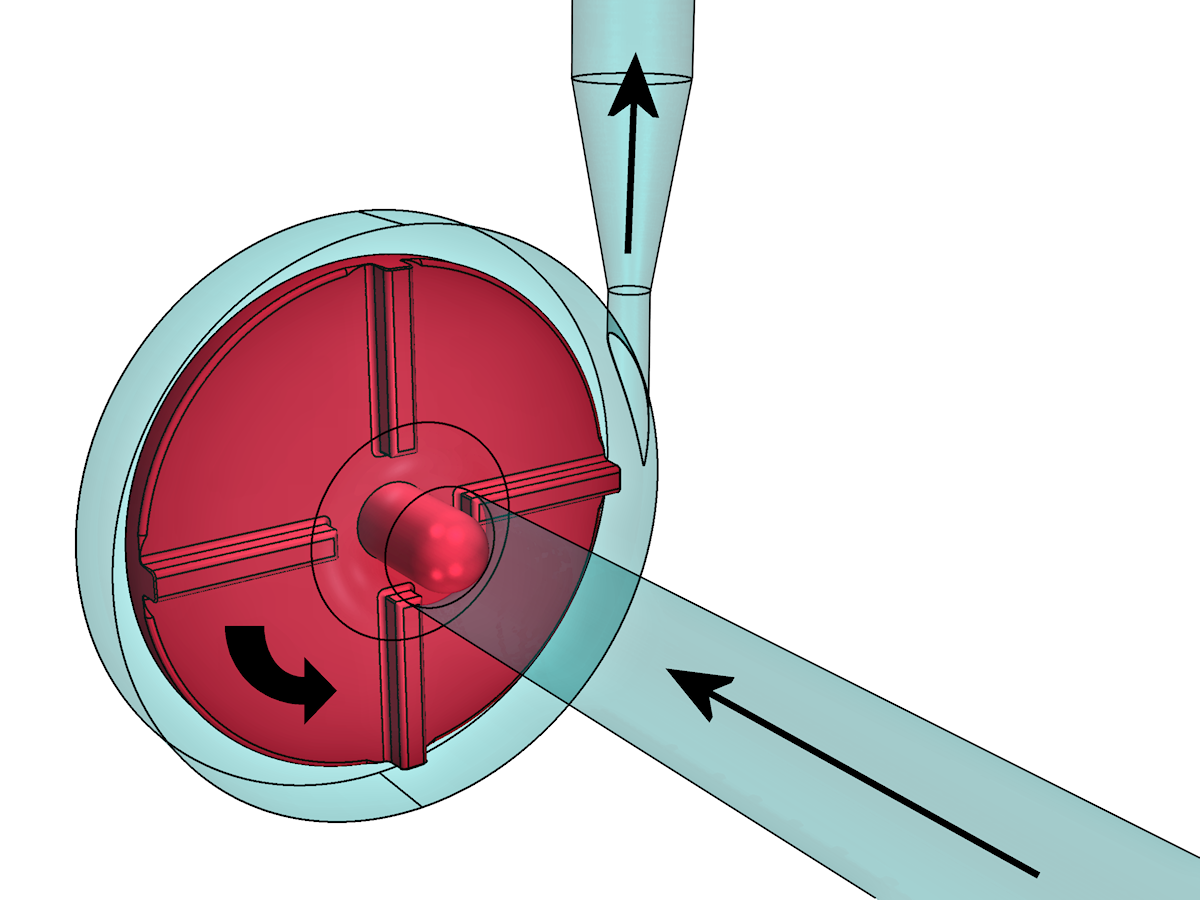
\includegraphics[width=3.2in]{imgs/nozzle_pump/housing_and_rotor.png}
    \end{minipage}
    \begin{minipage}[c][2.5in][c]{0.9\linewidth}
        \centering
        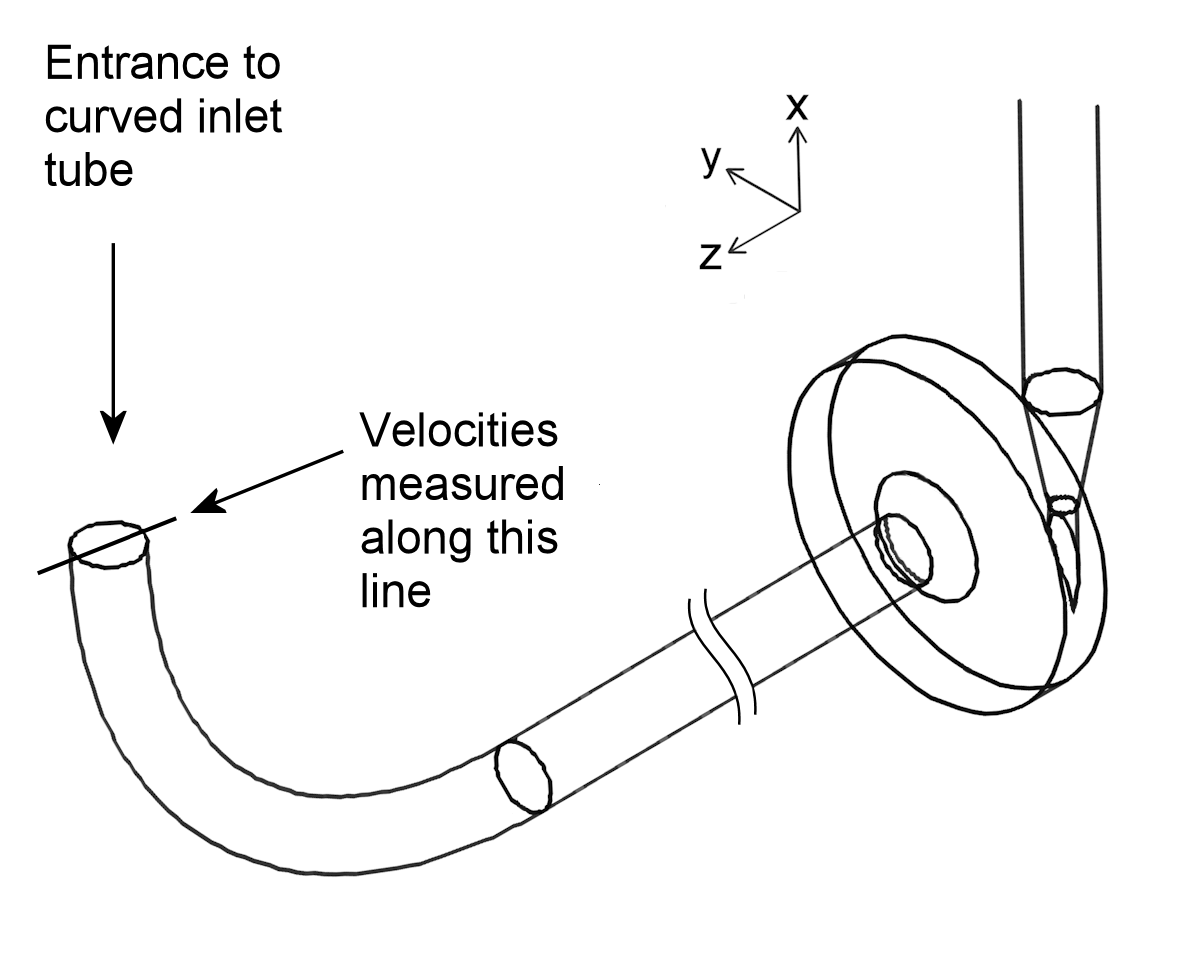
\includegraphics[width=3.2in]{imgs/nozzle_pump/inlet_velcocity_profile_location.png}
    \end{minipage}
    \caption{The geometry of and the flow direction in the blood pump (top), and the location where the velocity is measured in the experiments the velocity profile is prescribed in the simulations (right).}
    \label{fig:pumpgeo}
\end{figure}

%  pump simulation setup
As to the simulation set up, the velocity distribution is prescribed at the inlet (see figure~\ref{fig:pumpgeo} bottom plot), where the velocity profiles are obtained from the experimental measurements using PIV from \cite{cpi}. The pressure at the outlet is set to be constant, and the gravitational force is included. Since the goal is to predict the flow field after it reaching steady state, instead of letting the rotor rotate during simulation, the non-inertial reference frame is applied on the fluid around the rotor. This is because the flow around the rotor at steady state can be analogue to flow experiencing constant angular velocity. Using non-inertial reference frame avoids mesh distortion and frequent remeshing due to rotation. For turbulence model, the LES Smagorinsky sub-grid scale model is employed, with 7\% of turbulence intensity imposed at the inlet. 

[The simulation domain is decomposed into around 1 million tetrahedron elements as shown in figure ?.] 

% pump result
[Result]

% pump analysis
[Comparison]